\documentclass[]{article}

% Imported Packages
%------------------------------------------------------------------------------
\usepackage{amssymb}
\usepackage{amstext}
\usepackage{amsthm}
\usepackage{amsmath}
\usepackage{enumerate}
\usepackage{fancyhdr}
\usepackage[margin=1in]{geometry}
\usepackage{graphicx}
\usepackage{extarrows}
\usepackage{setspace}
\usepackage{float}
%------------------------------------------------------------------------------

% Header and Footer
%------------------------------------------------------------------------------
\pagestyle{plain}  
\renewcommand\headrulewidth{0.4pt}                                      
\renewcommand\footrulewidth{0.4pt}                                    
%------------------------------------------------------------------------------

% Title Details
%------------------------------------------------------------------------------
\title{Deliverable \#3 Template}
\author{SE 3A04: Software Design III -- Large System Design}
\date{}                               
%------------------------------------------------------------------------------

% Document
%------------------------------------------------------------------------------
\begin{document}

\maketitle	
\noindent{\bf Tutorial Number:} T01\\
{\bf Group Number:} G01 \\
{\bf Group Members:} 
\begin{itemize}
	\item Benjamin Bloomfield
	\item Vikram Chandar
    \item Trisha Panchal
    \item Yug Vashisth
    \item Hamza Nadeem
\end{itemize}

\newpage
\section{Introduction}
\label{sec:introduction}
% Begin Section

This section should provide an brief overview of the entire document.

\subsection{Purpose}
\label{sub:purpose}
% Begin SubSection
\begin{enumerate}[a)]
	\item Delineate the purpose of the document\\
    The purpose of this document is to provide further detail about the SCEMAS system, including State Charts for the Controller classes, Sequence Diagrams, and a detailed class diagram. A more detailed background of the SCEMAS system is provided in Deliverables 1 and 2.
	\item Specify the intended audience for the document\\
    The intended audience of this document is the stakeholders of SCEMAS, including developers, testers, and owners.
\end{enumerate}
% End SubSection

\subsection{System Description}
\label{sub:system_description}
% Begin SubSection
\begin{enumerate}[a)]
	\item Give a brief description of the system. This could be a paragraph or two to give some context to this document. \\
    The SCEMAS system is designed to share IoT data of sensors distributed across the city, acting as a monitoring network for an environmental monitoring system. The IoT sensors collect data, evaluate that data against thresholds, and send alerts when a threshold violation is detected so users can take any action needed. A dashboard is provided for city officials, while a public API will be provided for other users. The system is built using the PAC architecture that separates the interactive aspect of the system into a hierarchy of cooperating agents, each with its own logic and control component, complemented by the Repository architecture, which provides a centralized data store with consistent and uniform access mechanisms. 
\end{enumerate}
% End SubSection

\subsection{Overview}
\label{sub:overview}
% Begin SubSection
\begin{enumerate}[a)]
	\item Describe what the rest of the document contains\\
    Section 2 contains State Charts for each controller class specified in the analysis class diagram from Deliverable 2. Section 3 contains Sequence Diagrams for each business event from Deliverable 1. Section 4 contains a detailed UML class diagram.
	\item Explain how the document is organised \\
    The document is organized in a manner where it begins by showing state charts for each controller class of the system to help establish system behaviour. It then shows sequence diagrams for each use case, and finally provides a detailed class diagram of our system.
\end{enumerate}

% End SubSection

% End Section

\section{State Charts for Controller Classes}
\label{sec:state_charts_for_controller_classes}
% Begin Section
This section should provide a state chart for each controller class for your application.
% End Section

\begin{figure}[H]
    \centering
    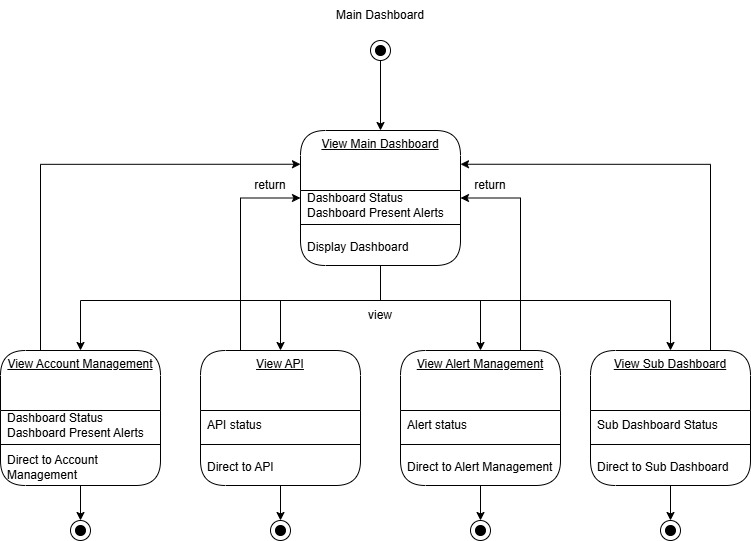
\includegraphics[width=1\textwidth]{./state_diagrams/Main Dashboard.jpg}
    \caption{State diagram for Main Dashboard Controller}
    \label{fig:analysis-class}
\end{figure}

\begin{figure}[H]
    \centering
    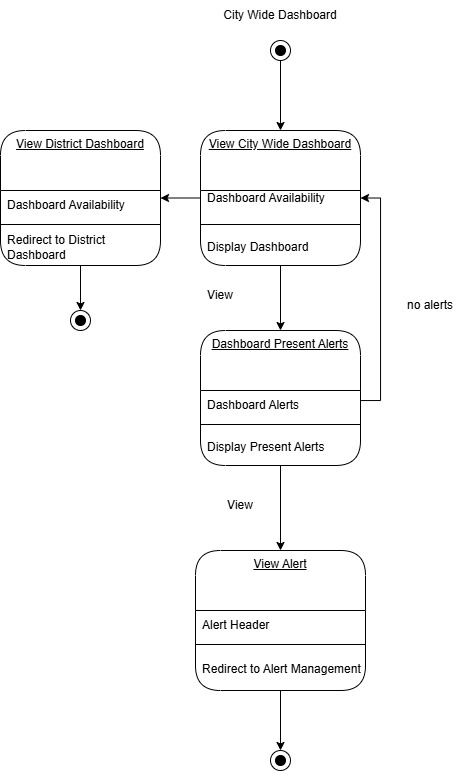
\includegraphics[width=0.5\textwidth]{./state_diagrams/City Dashboard.jpg}
    \caption{State diagram for City Dashboard Controller}
    \label{fig:analysis-class}
\end{figure}

\begin{figure}[H]
    \centering
    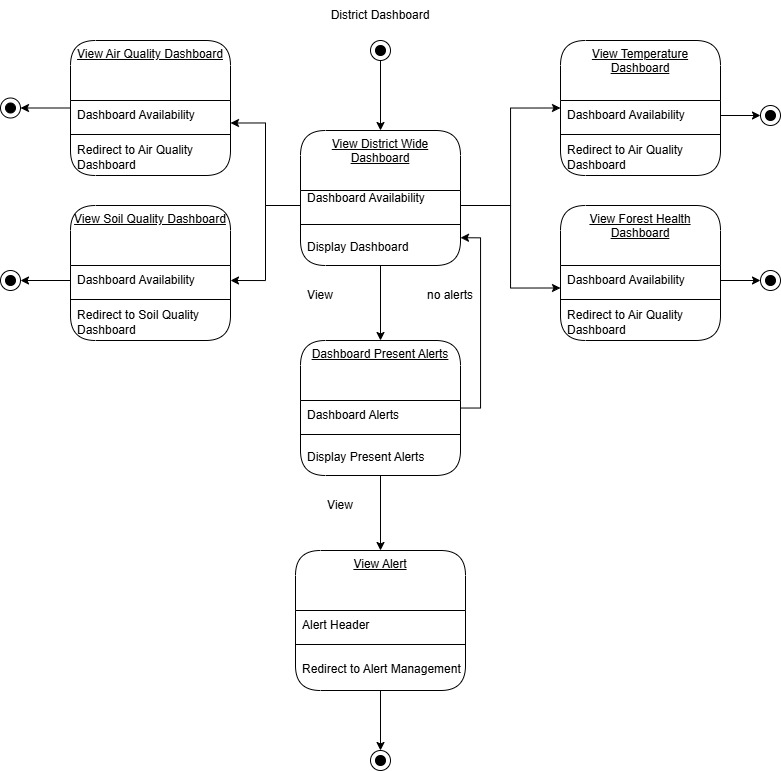
\includegraphics[width=1\textwidth]{./state_diagrams/District Dashboard.jpg}
    \caption{State diagram for District Dashboard Controller}
    \label{fig:analysis-class}
\end{figure}

\begin{figure}[H]
    \centering
    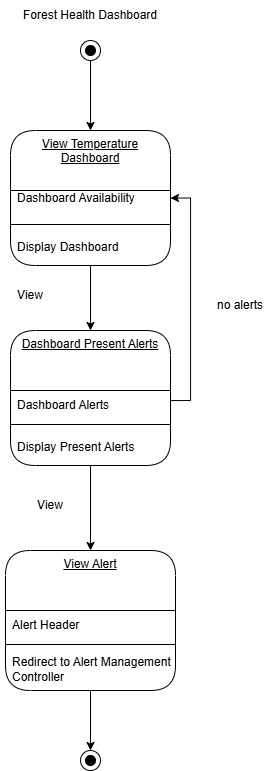
\includegraphics[width=0.4\textwidth]{./state_diagrams/Forest Health.jpg}
    \caption{State diagram for Forest Health Dashboard Controller}
    \label{fig:analysis-class}
\end{figure}

\begin{figure}[H]
    \centering
    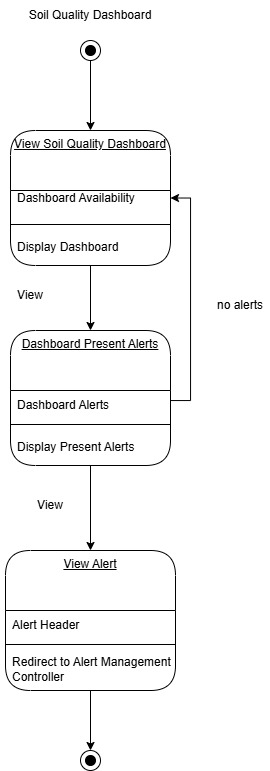
\includegraphics[width=0.4\textwidth]{./state_diagrams/Soil Quality.jpg}
    \caption{State diagram for Soil Quality Dashboard Controller}
    \label{fig:analysis-class}
\end{figure}

\begin{figure}[H]
    \centering
    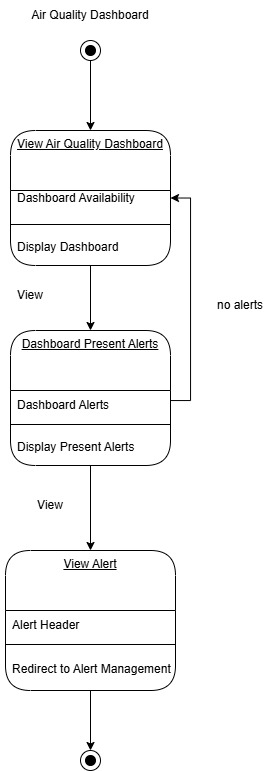
\includegraphics[width=0.4\textwidth]{./state_diagrams/Air Quality.jpg}
    \caption{State diagram for Air Quality Dashboard Controller}
    \label{fig:analysis-class}
\end{figure}

\begin{figure}[H]
    \centering
    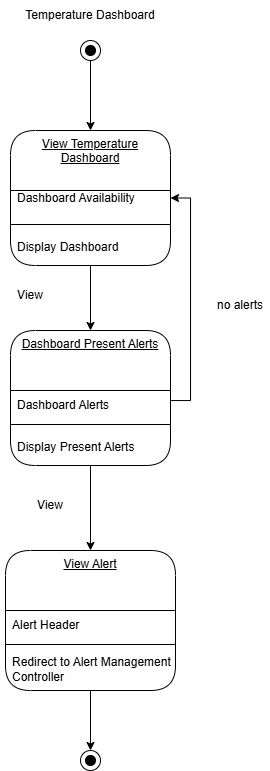
\includegraphics[width=0.4\textwidth]{./state_diagrams/Temperature Dashboard.jpg}
    \caption{State diagram for Temperature Dashboard Controller}
    \label{fig:analysis-class}
\end{figure}

\begin{figure}[H]
    \centering
    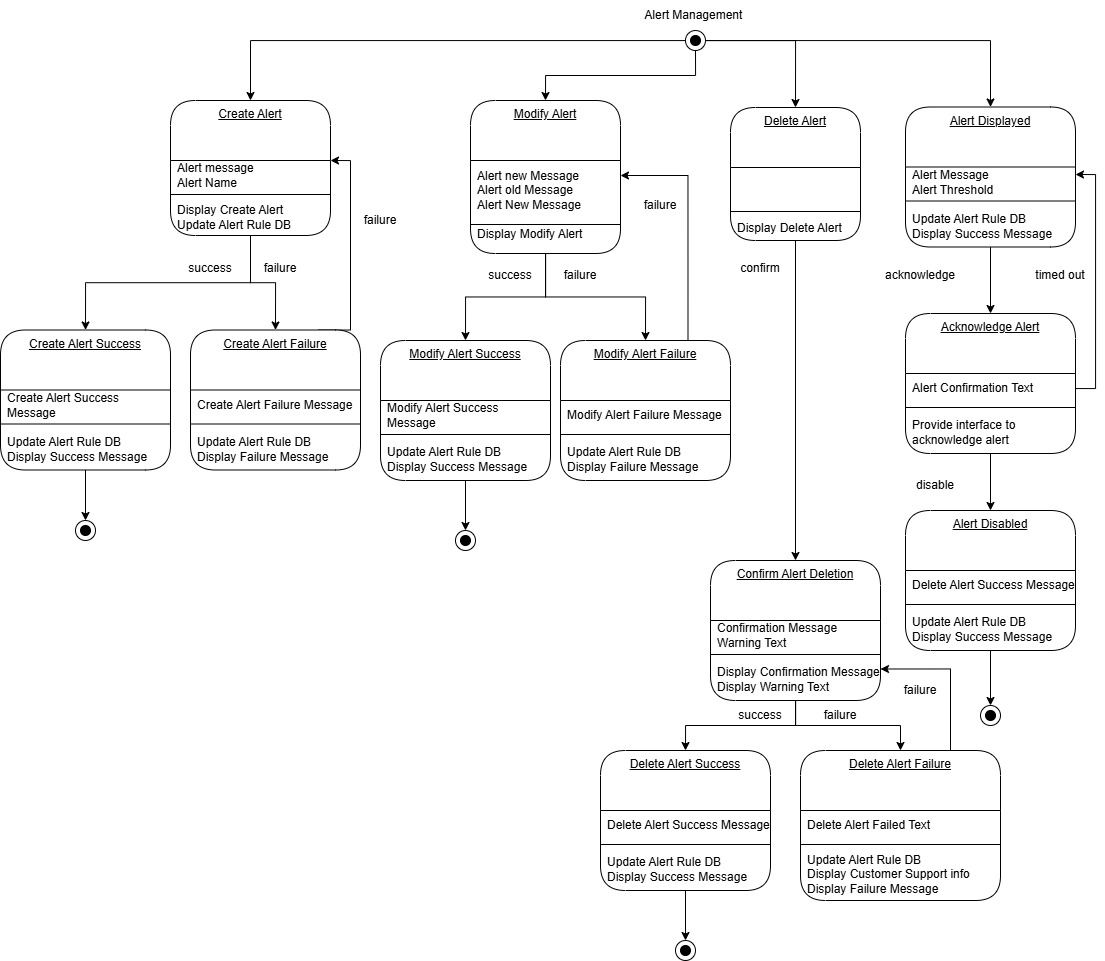
\includegraphics[width=1\textwidth]{./state_diagrams/Alert.jpg}
    \caption{State diagram for Alert Management Controller}
    \label{fig:analysis-class}
\end{figure}

\begin{figure}[H]
    \centering
    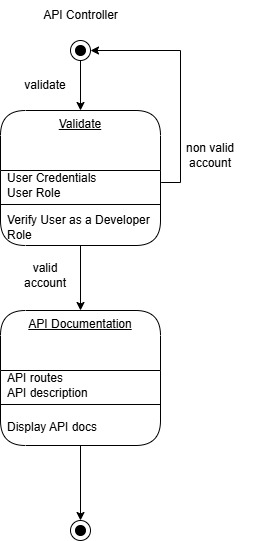
\includegraphics[width=0.4\textwidth]{./state_diagrams/API .jpg}
    \caption{State diagram for API Controller}
    \label{fig:analysis-class}
\end{figure}

\begin{figure}[H]
    \centering
    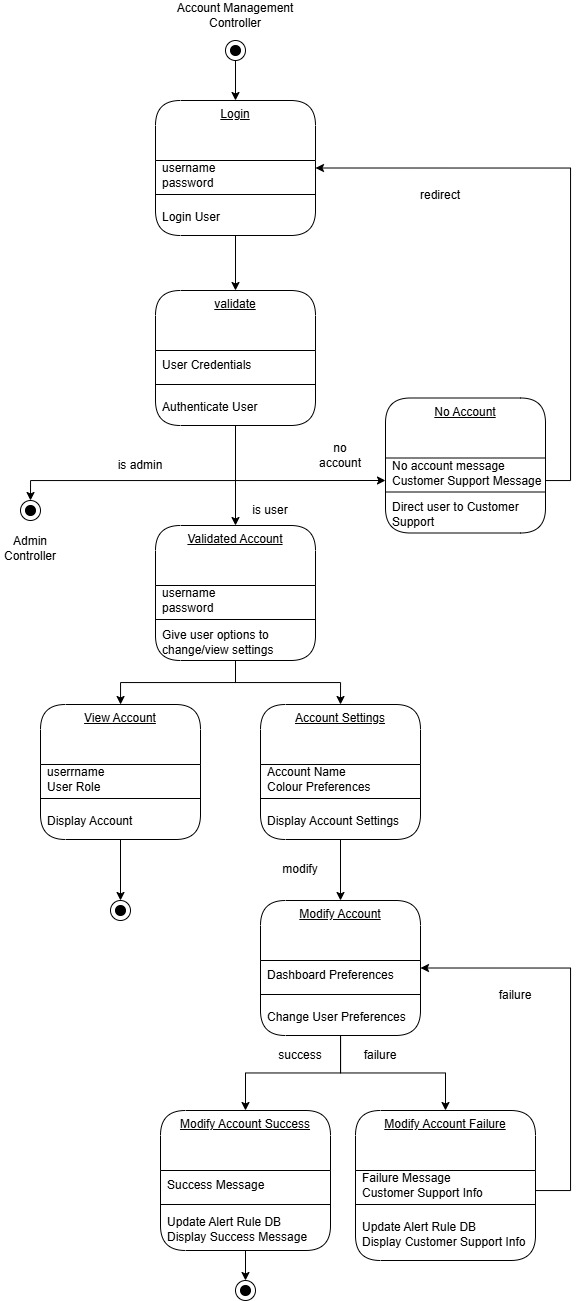
\includegraphics[width=0.5\textwidth]{./state_diagrams/Account.jpg}
    \caption{State diagram for Account Management Controller}
    \label{fig:analysis-class}
\end{figure}

\begin{figure}[H]
    \centering
    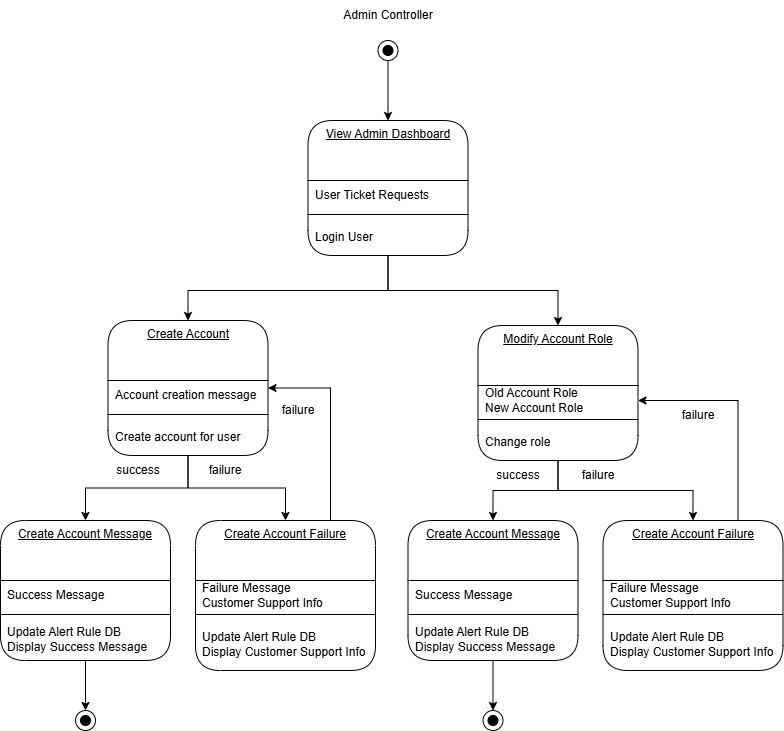
\includegraphics[width=1\textwidth]{./state_diagrams/Admin Controller.jpg}
    \caption{State diagram for Admin Controller}
    \label{fig:analysis-class}
\end{figure}

\section{Sequence Diagrams}
\label{sec:sequence_diagrams}
% Begin Section

\begin{figure}[H]
    \centering
    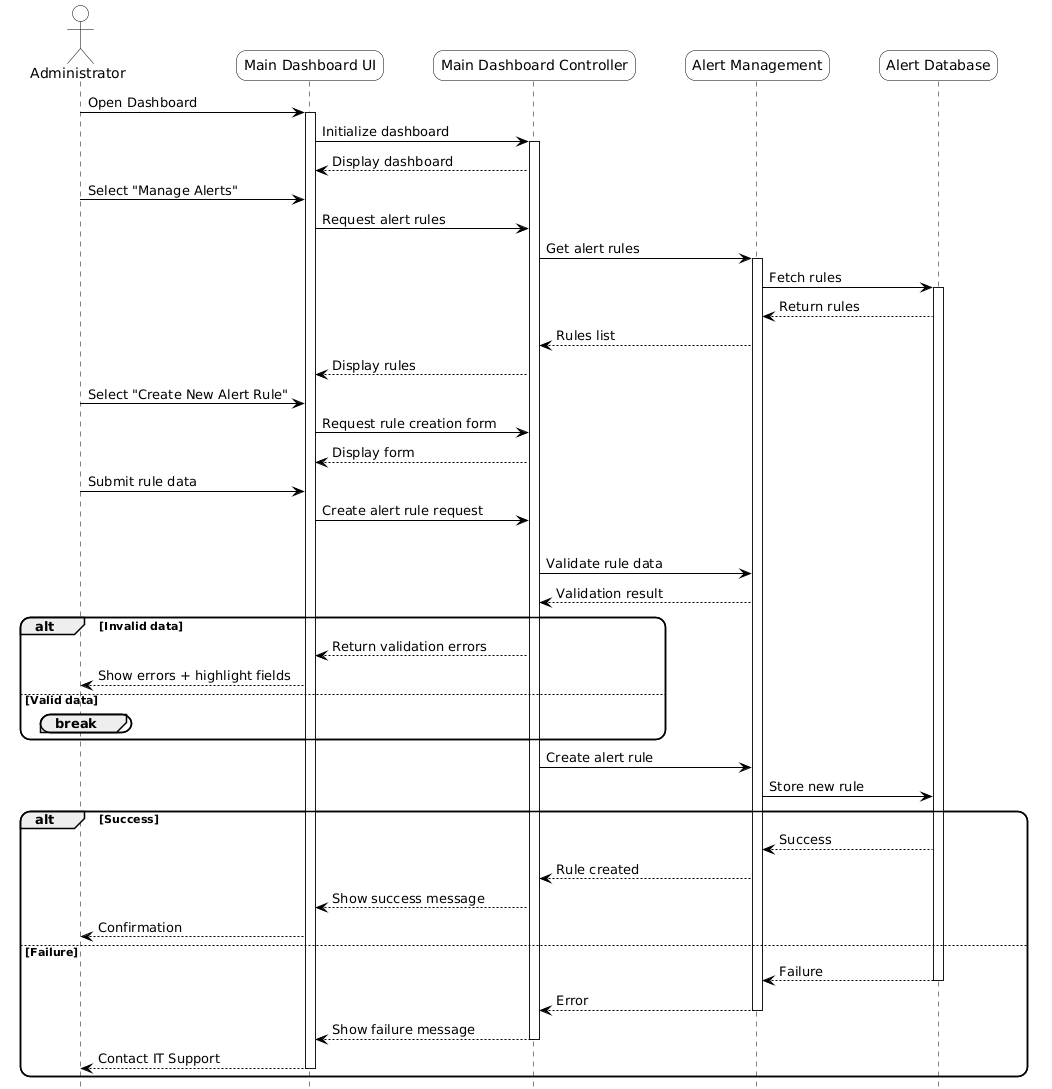
\includegraphics[width=1\textwidth]{./Sequence_Diagrams/SE_Create_Alert_Rule.png}
    \caption{Sequence diagram for creating a new alert rule}
    \label{fig:analysis-class}
\end{figure}

\begin{figure}[H]
    \centering
    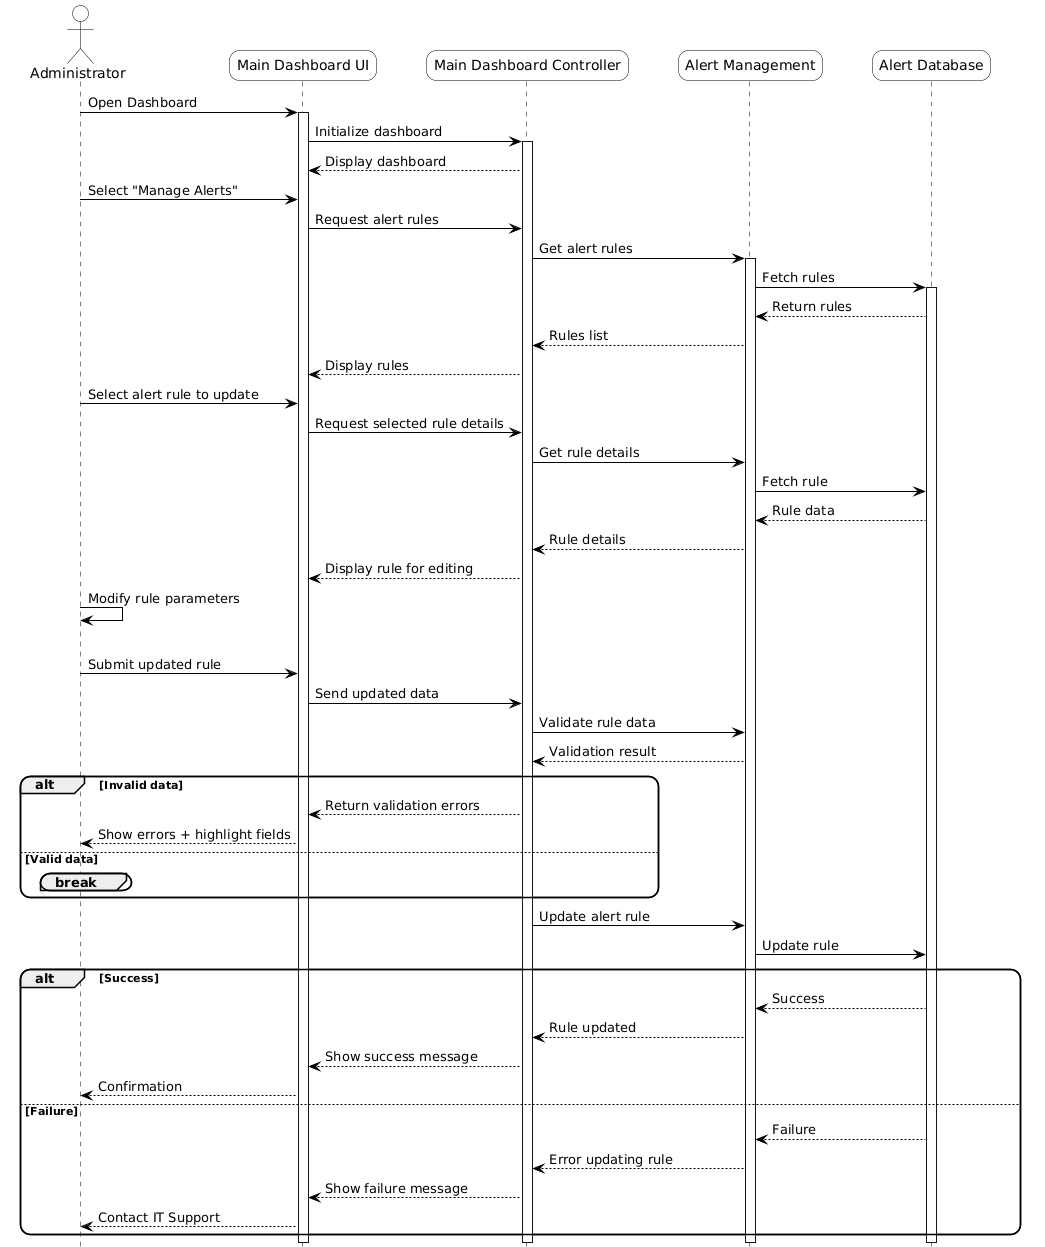
\includegraphics[width=1\textwidth]{./Sequence_Diagrams/SE_Update_Alert_Rule.png}
    \caption{Sequence diagram for updating an existing alert rule}
    \label{fig:analysis-class}
\end{figure}

\begin{figure}[H]
    \centering
    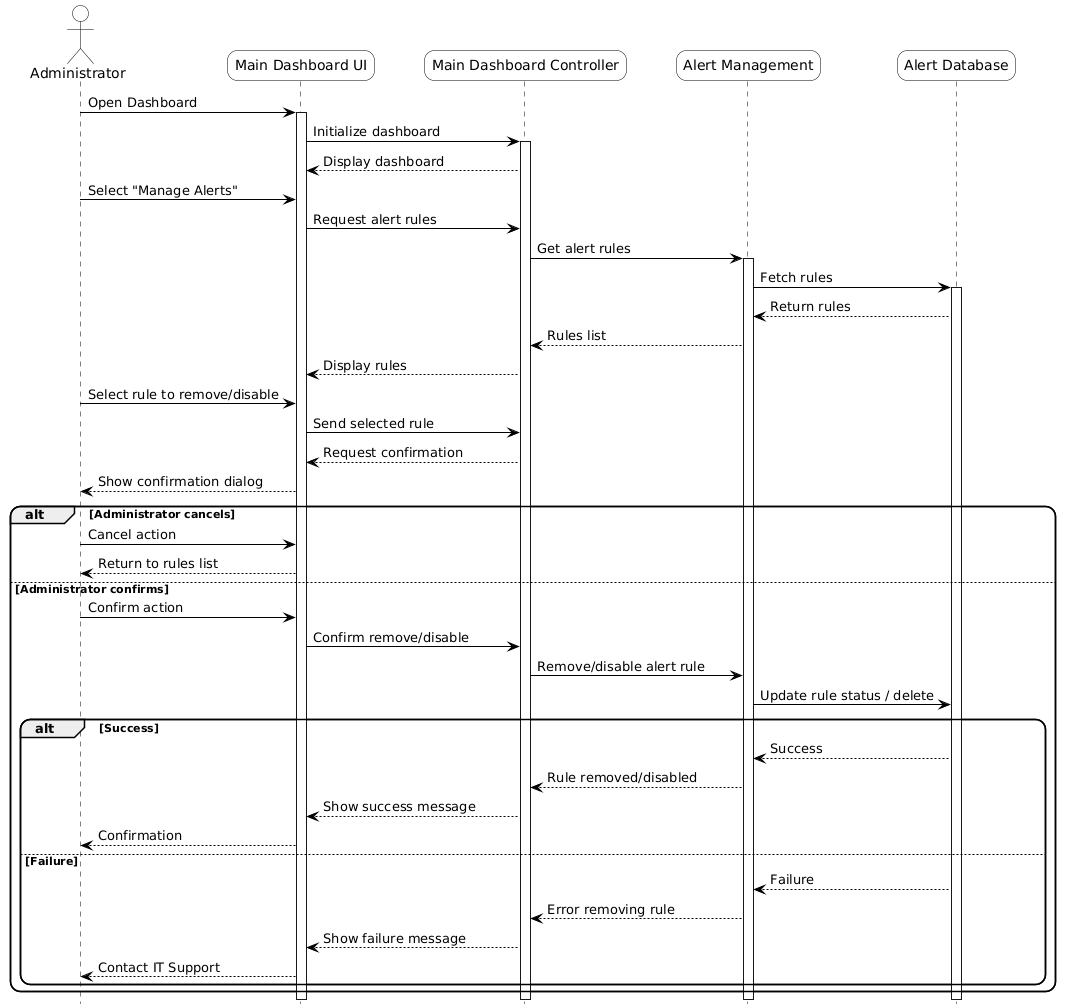
\includegraphics[width=1\textwidth]{./Sequence_Diagrams/SE_Remove_Alert_Rule.png}
    \caption{Sequence diagram for removing/disabling an existing alert rule}
    \label{fig:analysis-class}
\end{figure}

\begin{figure}[H]
    \centering
    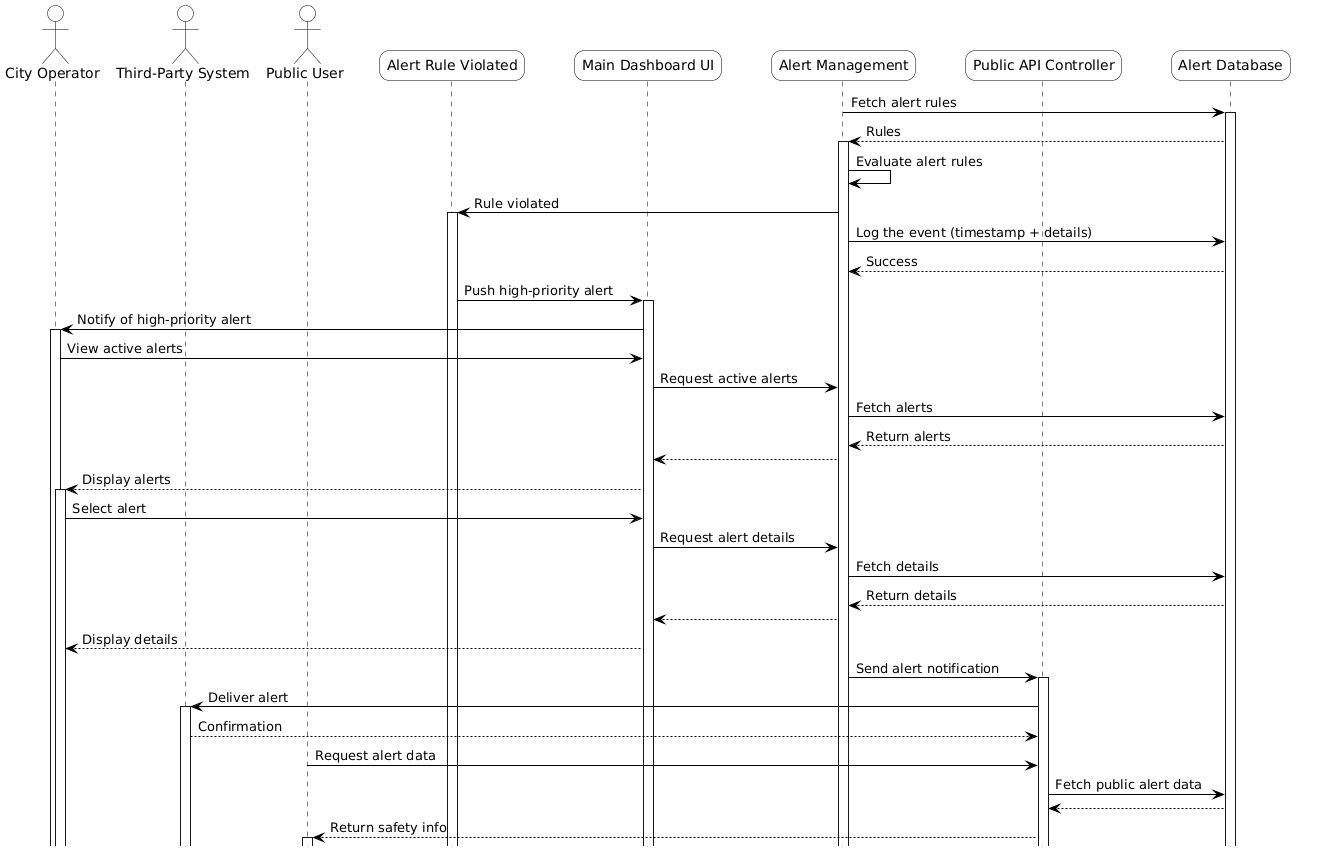
\includegraphics[width=1\textwidth]{./Sequence_Diagrams/SE_Rule_Violation_Detected.png}
    \caption{Sequence diagram for detecting a rule violation}
    \label{fig:analysis-class}
\end{figure}

\begin{figure}[H]
    \centering
    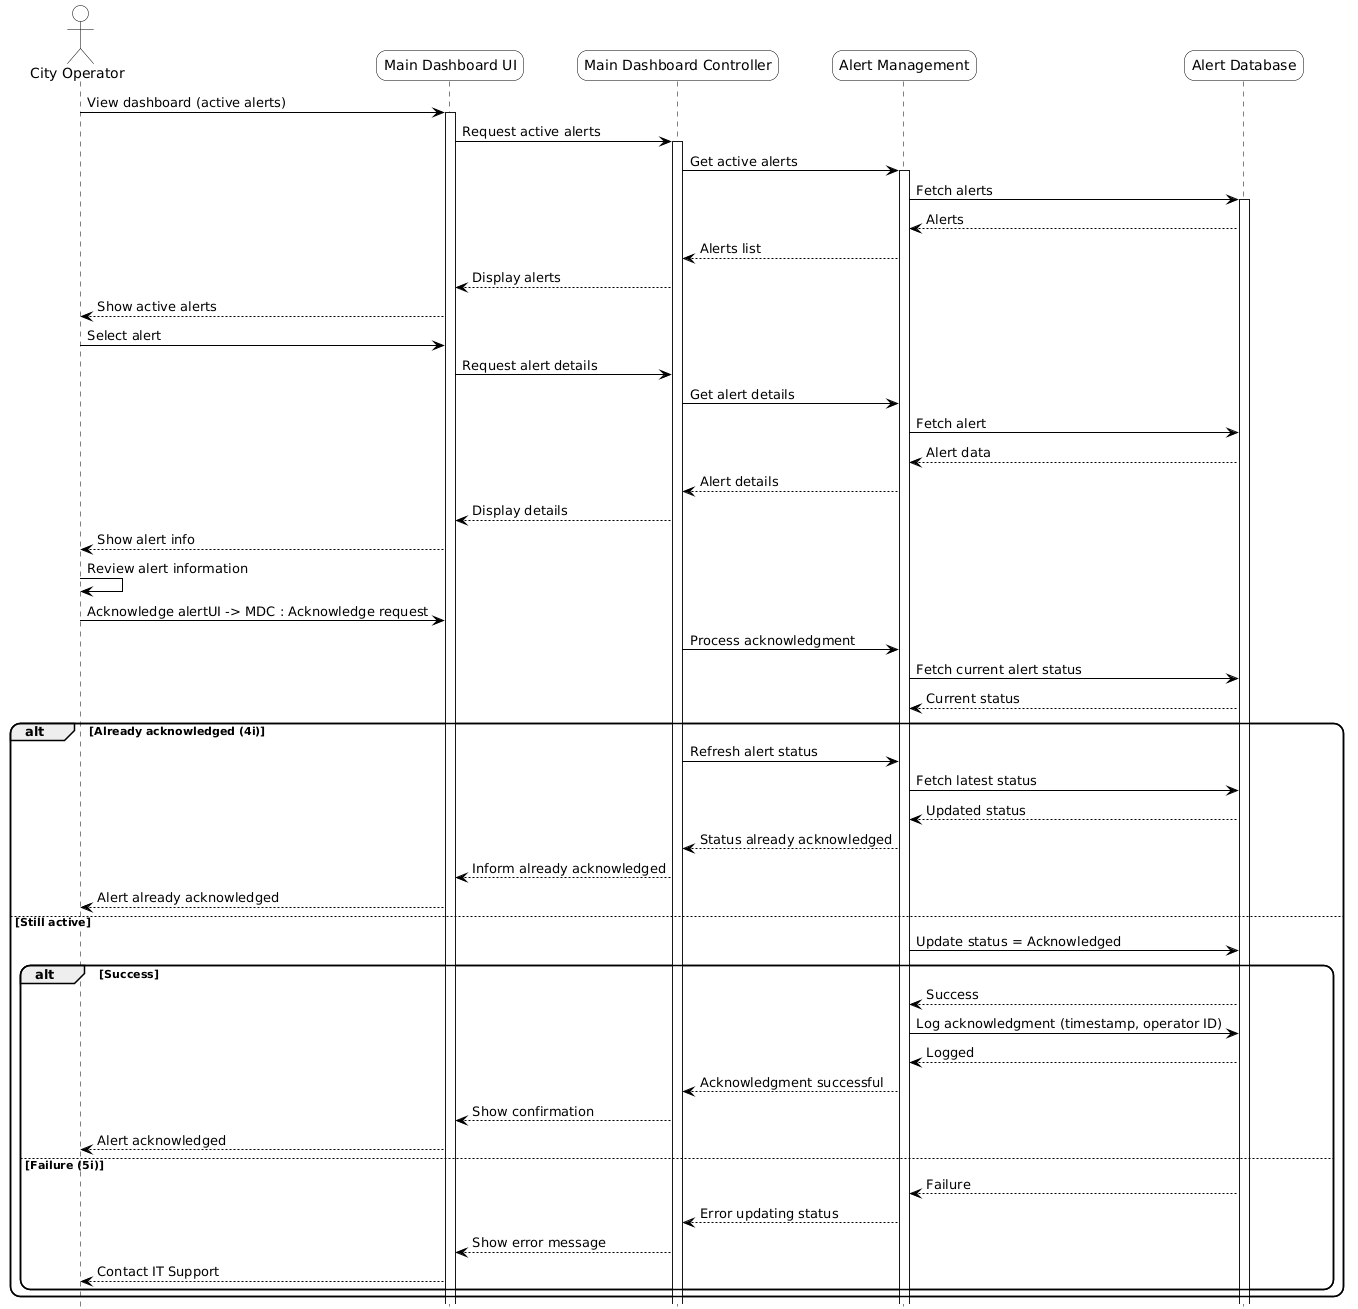
\includegraphics[width=1\textwidth]{./Sequence_Diagrams/SE_Alert_Acknowledged.png}
    \caption{Sequence diagram for acknowledging a rule violation}
    \label{fig:analysis-class}
\end{figure}
\begin{figure}[H]
    \centering
    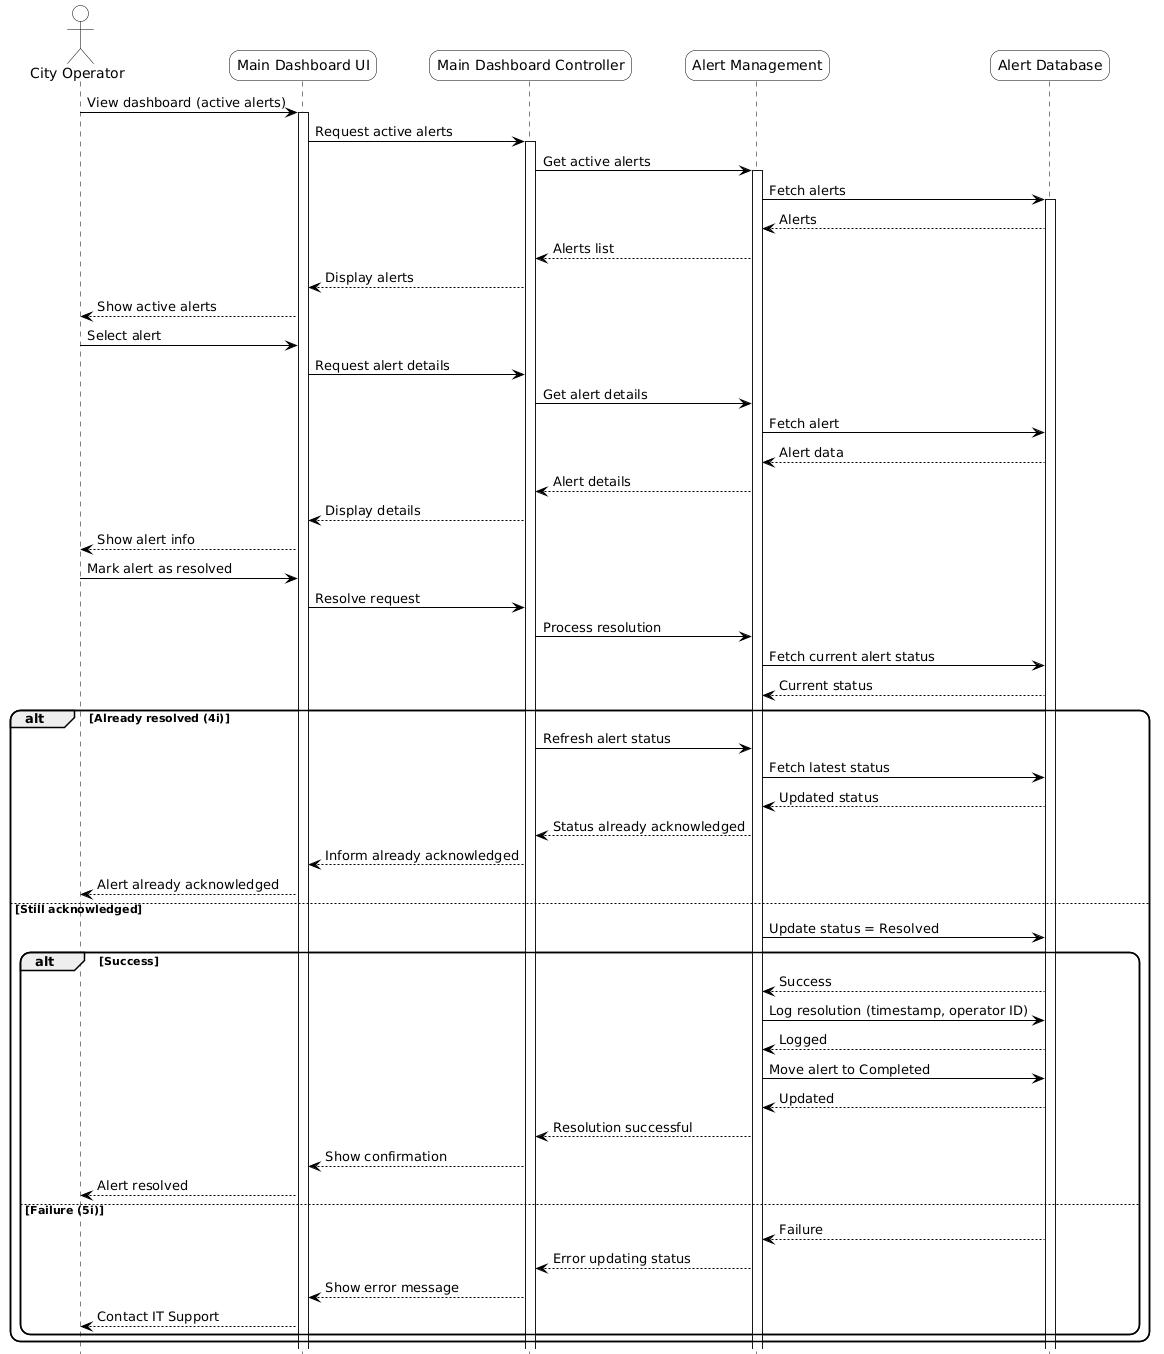
\includegraphics[width=1\textwidth]{./Sequence_Diagrams/SE_Alert_Resolved.png}
    \caption{Sequence diagram for resolving an alert rule violation}
    \label{fig:analysis-class}
\end{figure}

\begin{figure}[H]
    \centering
    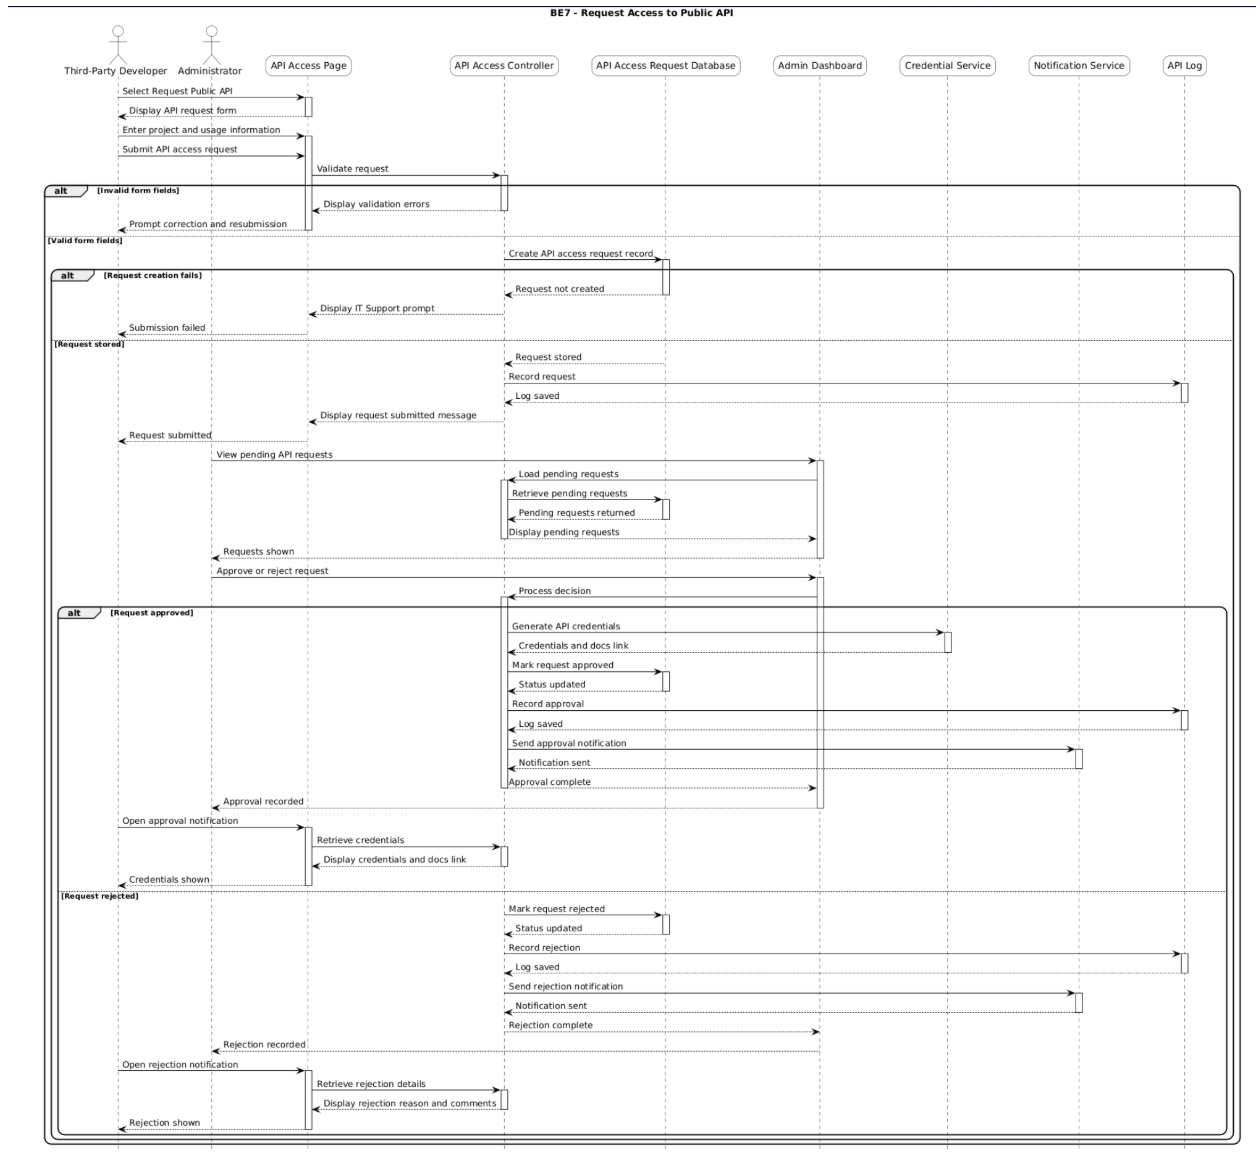
\includegraphics[width=1\textwidth]{./Sequence_Diagrams/BE7.png}
    \caption{Request access to public API}
    \label{fig:analysis-class}
\end{figure}
\begin{figure}[H]
    \centering
    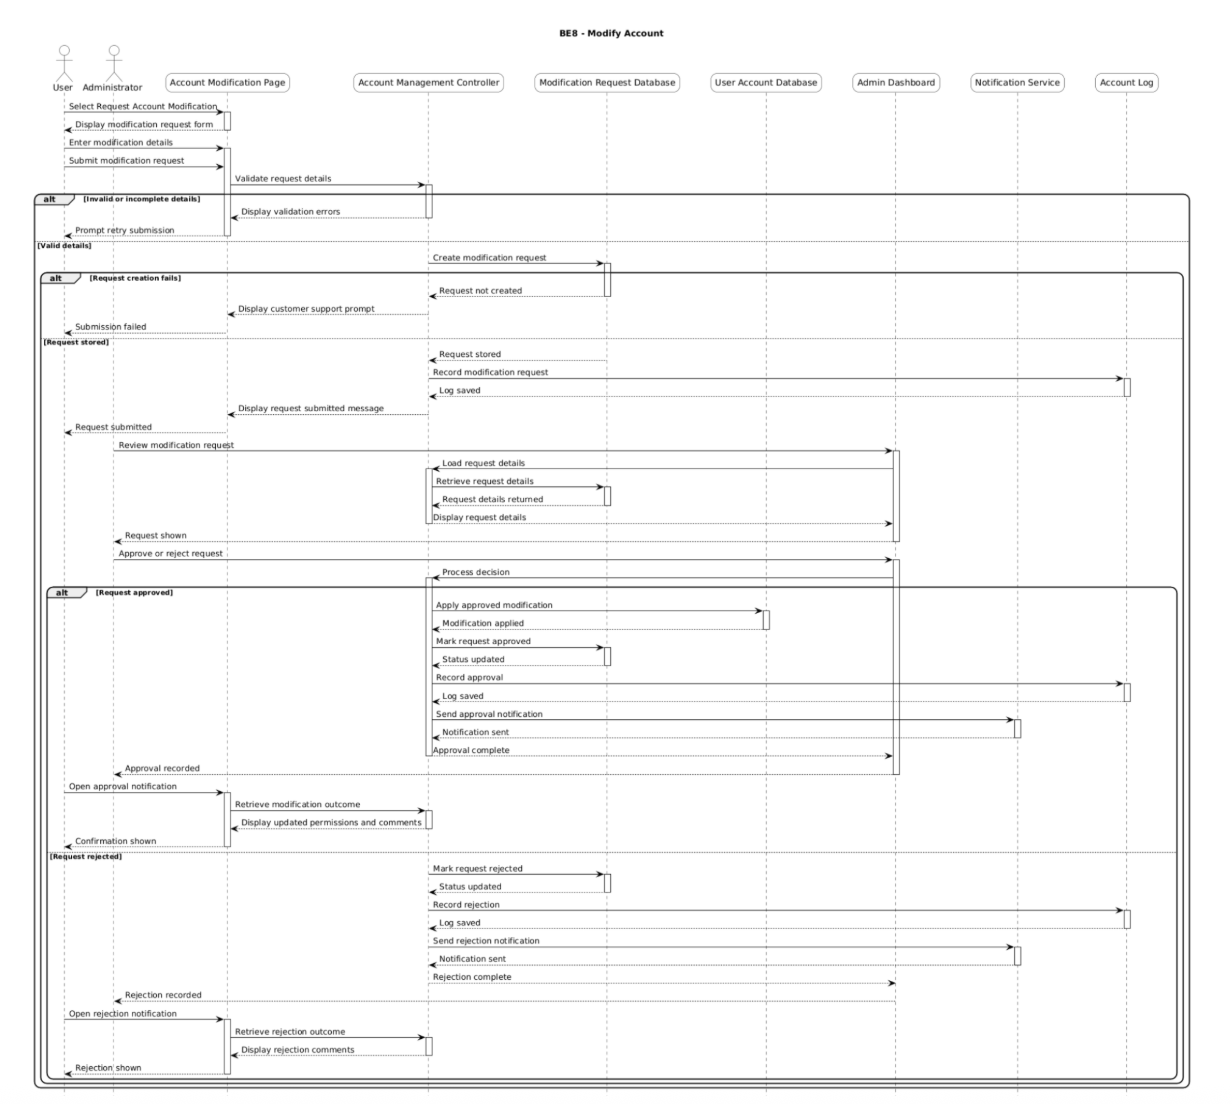
\includegraphics[width=1\textwidth]{./Sequence_Diagrams/BE8.png}
    \caption{Modify Account}
    \label{fig:analysis-class}
\end{figure}
\begin{figure}[H]
    \centering
    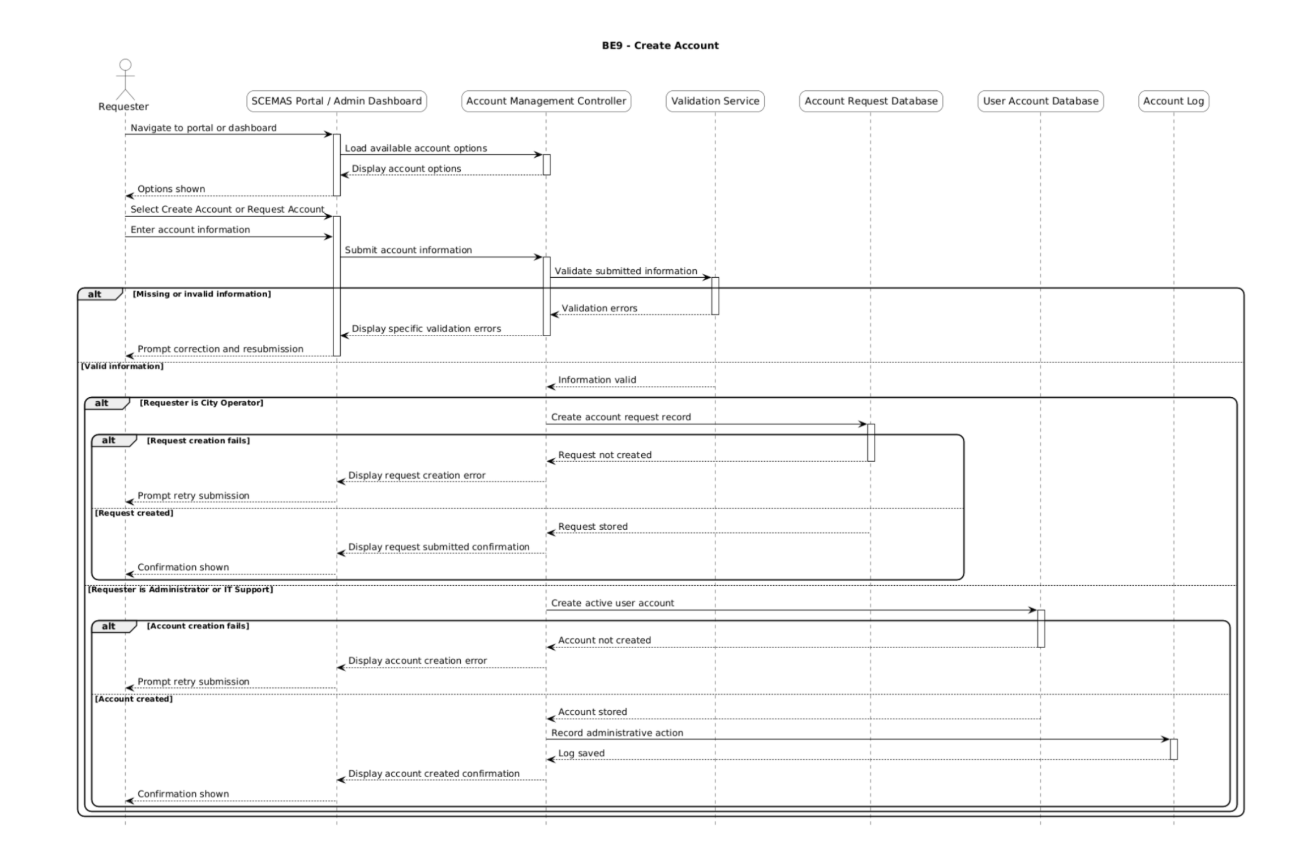
\includegraphics[width=1\textwidth]{./Sequence_Diagrams/BE9.png}
    \caption{Create Account}
    \label{fig:analysis-class}
\end{figure}
\begin{figure}[H]
    \centering
    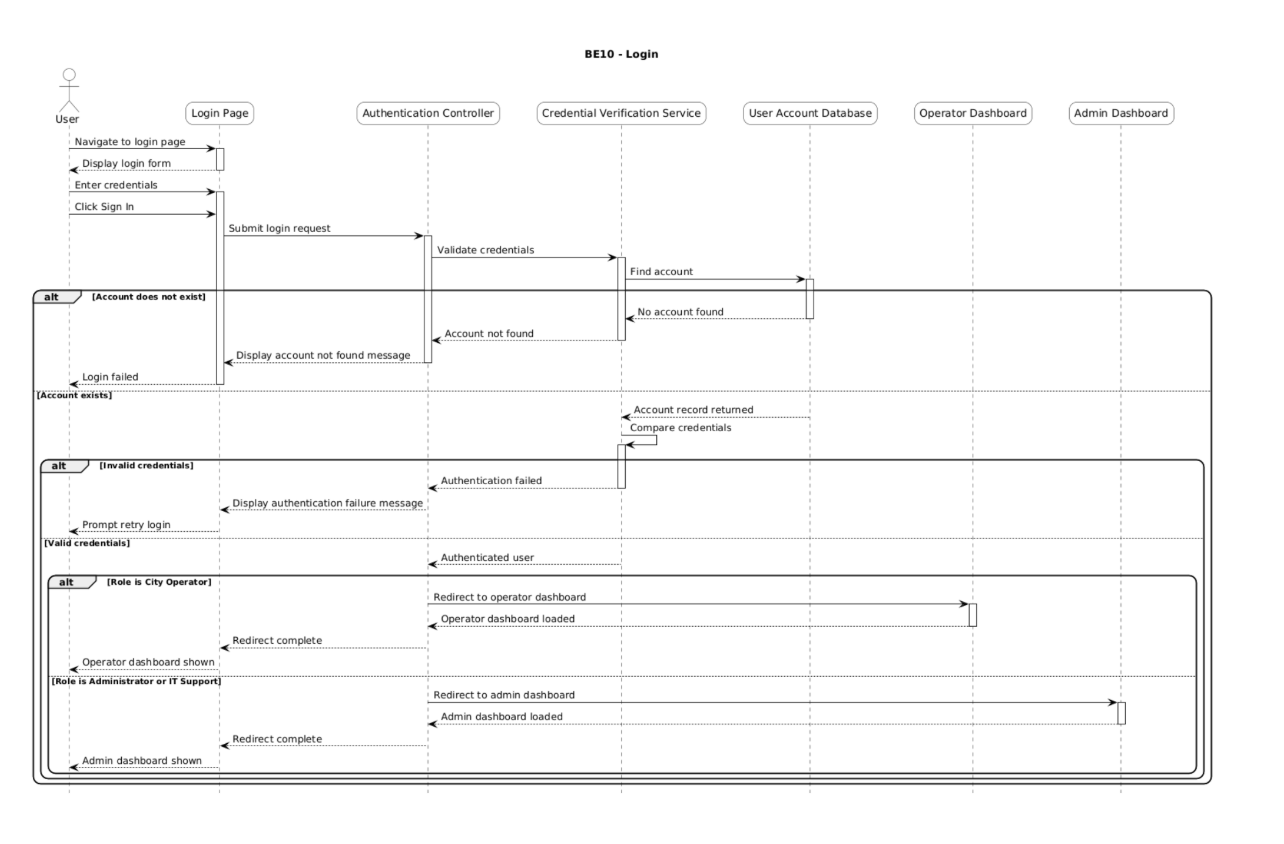
\includegraphics[width=1\textwidth]{./Sequence_Diagrams/BE10.png}
    \caption{Login}
    \label{fig:analysis-class}
\end{figure}

%End Section

\section{Detailed Class Diagram}
\label{sec:detailed_class_diagram}
% Begin Section
This section provides a detailed class diagram for SCEMAS.
\begin{figure}[H]
    \centering
    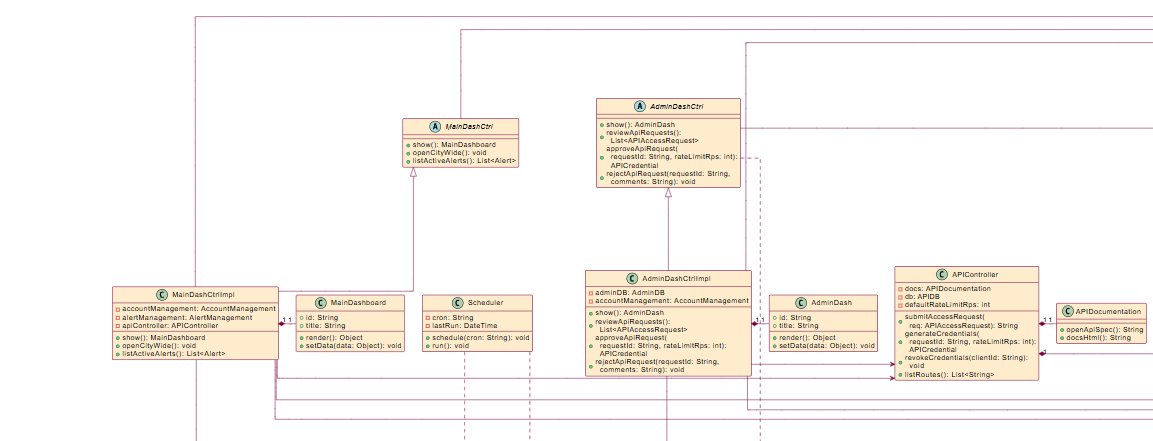
\includegraphics[width=1\textwidth]{./class-diagrams/UML1.png}
    \caption{Top-left of UML Class Diagram}
    \label{fig:full-class-diagram}
\end{figure}
\begin{figure}[H]
    \centering
    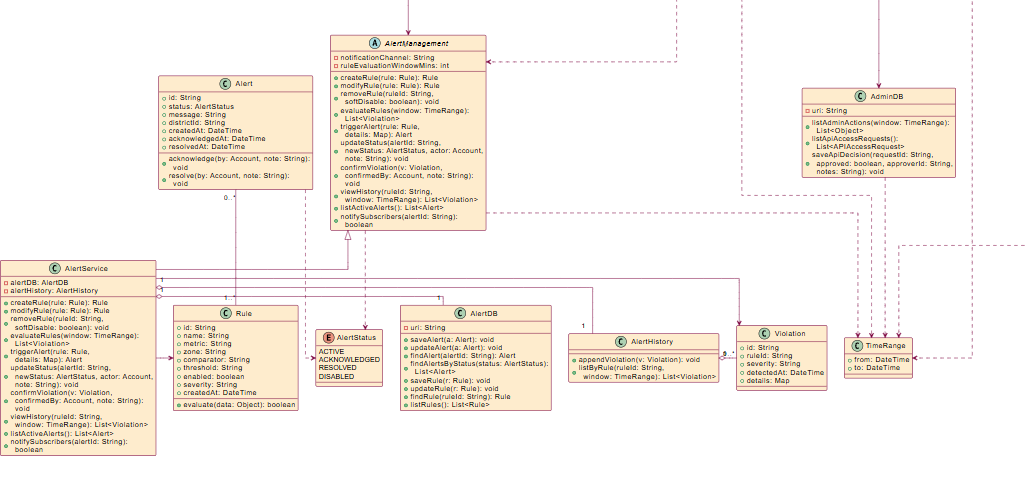
\includegraphics[width=1\textwidth]{./class-diagrams/UML2.png}
    \caption{Bottom-Left of UML Class Diagram}
    \label{fig:full-class-diagram}
\end{figure}
\begin{figure}[H]
    \centering
    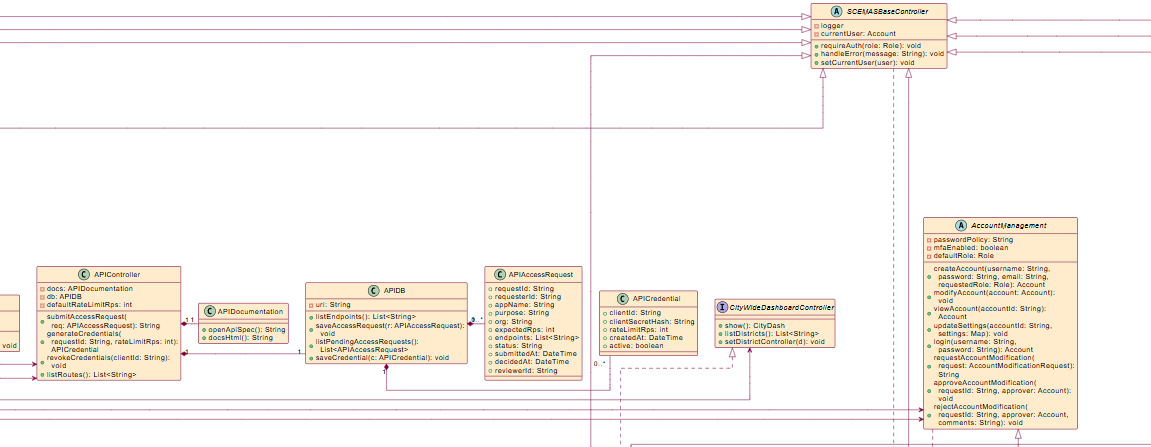
\includegraphics[width=1\textwidth]{./class-diagrams/UML3.png}
    \caption{Middle-Top of UML Class Diagram}
    \label{fig:full-class-diagram}
\end{figure}
\begin{figure}[H]
    \centering
    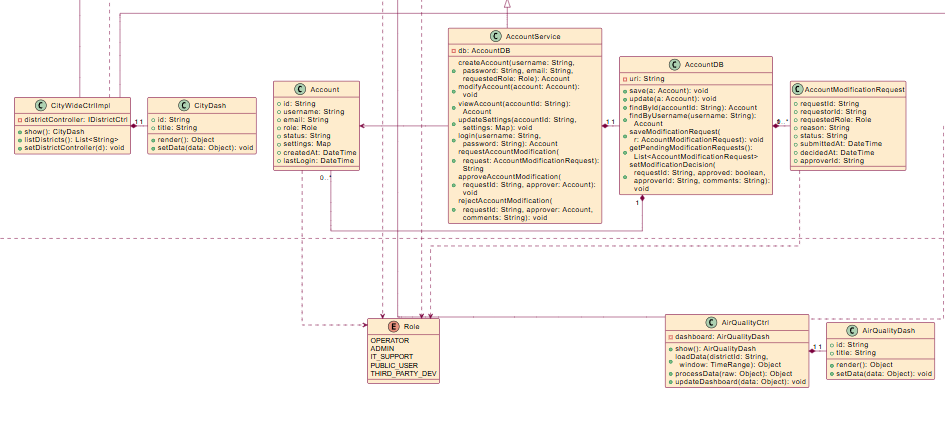
\includegraphics[width=1\textwidth]{./class-diagrams/UML4.png}
    \caption{Middle-Bottom of UML Class Diagram}
    \label{fig:full-class-diagram}
\end{figure}
\begin{figure}[H]
    \centering
    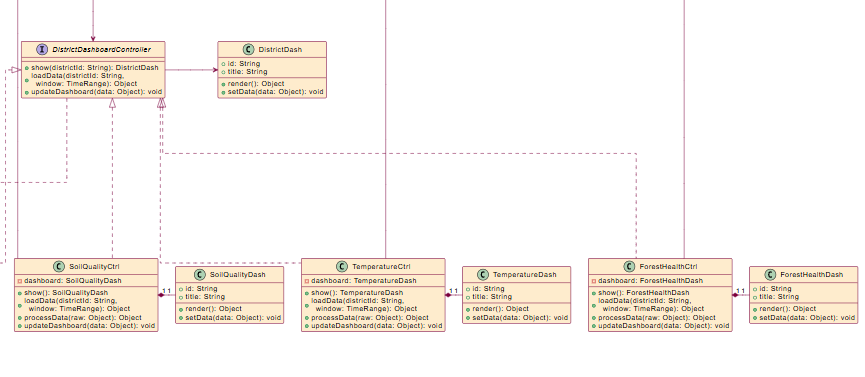
\includegraphics[width=1\textwidth]{./class-diagrams/UML5.png}
    \caption{Bottom-Right of UML Class Diagram}
    \label{fig:full-class-diagram}
\end{figure}
% End Section

\appendix
\section{Division of Labour}
\label{sec:division_of_labour}
% Begin Section
Include a Division of Labour sheet which indicates the contributions of each team member. This sheet must be signed by all team members.
% End Section

\newpage
\appendix
\section{Division of Labour}
\label{sec:division_of_labour}
% Begin Section

\noindent \textbf{Benjamin Bloomfield} 
\begin{itemize}
    \item Sequence Diagrams 1-6
	\item Document organization 

    \vspace{0.5cm}
    \centering
    
\includegraphics[width=10cm]{./signatures/ben_bloomfield_signature.jpg}
    \\\vspace{0.2cm}
    Date: March 22nd, 2026
    \vspace{0.5cm}
\end{itemize}


\noindent \textbf{Vikram Chandar}
\begin{itemize}
    \item State Diagrams 1-11
    
    \vspace{0.5cm}
    \centering
    \vspace{2cm}
    
\includegraphics[width=10cm]{./signatures/IMG_4568.jpg}
    \\\vspace{0.2cm}
    Date: March 22nd, 2026 
    \vspace{0.5cm}
\end{itemize}


\noindent \textbf{Trisha Panchal}
\begin{itemize}
    \item Section 4:
    \begin{itemize}
        \item Discussed key classes and their responsibilities with Hamza.
        \item Identified components of the detailed class diagram (deciding concrete and abstract classes and interfaces).
        \item Designed skeleton for class diagram in PlantUML.
        \item Added attributes with access modifiers and types.
        \item Added methods with access modifiers, and refined to have appropriate return types and parameters.
        \item Added relationships between components, identifying associations and multiplicities.
    \end{itemize}
    \vspace{0.5cm}
    \centering
    
\includegraphics[width=10cm]{./signatures/trisha_d1_sign.jpg}
    \\\vspace{0.2cm}
    Date: March 22nd, 2026
    \vspace{0.5cm}
\end{itemize}


\noindent \textbf{Yug Vashisth}
\begin{itemize}
    \item Sequence Diagrams 5, 7-10
    \vspace{0.5cm}
        \centering
        
\includegraphics[width=10cm]{./signatures/yug_sig.jpg}
        \\\vspace{0.2cm}
        Date: March 22nd, 2026
    \vspace{0.5cm}	
\end{itemize}


\noindent \textbf{Hamza Nadeem}
\begin{itemize}
    \item Section 1: Introduction
    \item Section 4: Detailed Class Diagram
    \begin{itemize}
        \item Assisted in planning the class diagram
        \item reviewed the class diagram
    \end{itemize}

    \vspace{0.5cm}
    \centering
    
\includegraphics[width=5cm]{signatures/hamza_nadeem_signature.jpeg}
    \\\vspace{0.2cm}
    Date: March 22nd, 2026
    \vspace{0.5cm} 
\end{itemize}


\end{document}
%------------------------------------------------------------------------------